\documentclass[12pt,twoside]{article}
%%%%%%%%%%%%%%%%%%%%%%%%%%%%%%%%%%%%%%%%%%%%%%%%%%%%%%%%%%%%%
% Meta informations:
\newcommand{\trauthor}{Klaus Ziegert, Jose Rodriguez Parra}
\newcommand{\trtype}{Seminararbeit} %{Seminararbeit} %{Proseminararbeit}
\newcommand{\trcourse}{Integration Komplexe Information Systeme}
\newcommand{\trtitle}{Time Series Data Cleaning: From Anomaly Detection to
Anomaly Repairing}
\newcommand{\trarbeitsbereich}{Datenbanken und Information Systeme}
\newcommand{\trdate}{\today}
%%%%%%%%%%%%%%%%%%%%%%%%%%%%%%%%%%%%%%%%%%%%%%%%%%%%%%%%%%%%
% Languages:
\usepackage[utf8]{inputenc}
\usepackage[ngerman]{babel}
\usepackage[numbers]{natbib}
%%%%%%%%%%%%%%%%%%%%%%%%%%%%%%%%%%%%%%%%%%%%%%%%%%%%%%%%%%%%%
% Bind packages:
\usepackage{tikz}
\usepackage{pgfplots}
\usepackage{acronym}                    % Acronyms
\usepackage{algorithmic}								% Algorithms and Pseudocode
\usepackage{algorithm}									% Algorithms and Pseudocode
\usepackage{amsfonts}                   % AMS Math Packet (Fonts)
\usepackage{amsmath}                    % AMS Math Packet
\usepackage{amssymb}                    % Additional mathematical symbols
\usepackage{amsthm}
\usepackage{booktabs}                   % Nicer tables
%\usepackage[font=small,labelfont=bf]{caption} % Numbered captions for figures
\usepackage{color}                      % Enables defining of colors via \definecolor
\definecolor{uhhRed}{RGB}{254,0,0}		  % Official Uni Hamburg Red
\definecolor{uhhGrey}{RGB}{122,122,120} % Official Uni Hamburg Grey
\usepackage{fancybox}                   % Gleichungen einrahmen
\usepackage{fancyhdr}										% Packet for nicer headers
%\usepackage{fancyheadings}             % Nicer numbering of headlines

%\usepackage[outer=3.35cm]{geometry} 	  % Type area (size, margins...) !!!Release version
%\usepackage[outer=2.5cm]{geometry} 		% Type area (size, margins...) !!!Print version
%\usepackage{geometry} 									% Type area (size, margins...) !!!Proofread version
\usepackage[outer=3.3cm]{geometry} 	  % Type area (size, margins...) !!!Draft version
\geometry{a4paper,body={5.8in,9in}}

\usepackage{graphicx}                   % Inclusion of graphics
%\usepackage{latexsym}                  % Special symbols
\usepackage{longtable}									% Allow tables over several parges
\usepackage{listings}                   % Nicer source code listings
\usepackage{multicol}										% Content of a table over several columns
\usepackage{multirow}										% Content of a table over several rows
\usepackage{rotating}										% Alows to rotate text and objects
\usepackage[hang]{subfigure}            % Allows to use multiple (partial) figures in a fig
%\usepackage[font=footnotesize,labelfont=rm]{subfig}	% Pictures in a floating environment

\usepackage{tabularx}										% Tables with fixed width but variable rows
\usepackage{url,xspace,boxedminipage}   % Accurate display of URLs
\usepackage[font=small,labelfont=bf]{caption}
% subcaption broke
% \usepackage{subcaption}
\usepackage{placeins} %need floatbarriers
%\usepackage[toc,symbols,nomain]{glossaries} %glossary
%%%% PHRI PACKAGES %%%%%
\usepackage{svg}
\usepackage{pdfpages} %for inserting pdfs
%%%%%%%%%%%%%%%%%%%%%%%%%%%%%%%%%%%%%%%%%%%%%%%%%%%%%%%%%%%%%
% Configurationen:

\hyphenation{whe-ther} 									% Manually use: "\-" in a word: Staats\-ver\-trag

%\lstloadlanguages{C}                   % Set the default language for listings
\DeclareGraphicsExtensions{.pdf,.svg,.jpg,.png,.eps} % first try pdf, then eps, png and jpg
\graphicspath{{./src/}} 								% Path to a folder where all pictures are located
\pagestyle{fancy} 											% Use nicer header and footer

% Redefine the environments for floating objects:
\setcounter{topnumber}{3}
\setcounter{bottomnumber}{2}
\setcounter{totalnumber}{4}
\renewcommand{\topfraction}{0.9} 			  %Standard: 0.7
\renewcommand{\bottomfraction}{0.5}		  %Standard: 0.3
\renewcommand{\textfraction}{0.1}		  	%Standard: 0.2
\renewcommand{\floatpagefraction}{0.8} 	%Standard: 0.5

% Tables with a nicer padding:
\renewcommand{\arraystretch}{1.2}

%%%%%%%%%%%%%%%%%%%%%%%%%%%%
% Additional 'theorem' and 'definition' blocks:
\theoremstyle{plain}
% \newtheorem{theorem}{Theorem}[section]
\newtheorem{theorem}{Satz}[section]		% Wenn in Deutsch geschrieben wird.
\newtheorem{axiom}{Axiom}[section] 	
%\newtheorem{axiom}{Fakt}[chapter]			% Wenn in Deutsch geschrieben wird.
%Usage:%\begin{axiom}[optional description]%Main part%\end{fakt}

\theoremstyle{definition}
\newtheorem{definition}{Definition}[section]

%Additional types of axioms:
\newtheorem{lemma}[axiom]{Lemma}
\newtheorem{observation}[axiom]{Observation}

%Additional types of definitions:
\theoremstyle{remark}
%\newtheorem{remark}[definition]{Bemerkung} % Wenn in Deutsch geschrieben wird.
\newtheorem{remark}[definition]{Remark} 

%%%%%%%%%%%%%%%%%%%%%%%%%%%%
% Provides TODOs within the margin:
\newcommand{\TODO}[1]{\marginpar{\emph{\small{{\bf TODO:} #1}}}}

%%%%%%%%%%%%%%%%%%%%%%%%%%%%
% Abbreviations and mathematical symbols
\newcommand{\modd}{\text{mod}}
\newcommand{\RS}{\mathbb{R}}
\newcommand{\NS}{\mathbb{N}}
\newcommand{\ZS}{\mathbb{Z}}
\newcommand{\dnormal}{\mathit{N}}
\newcommand{\duniform}{\mathit{U}}

\newcommand{\erdos}{Erd\H{o}s}
\newcommand{\renyi}{-R\'{e}nyi}
%%%%%%%%%%%%%%%%%%%%%%%%%%%%%%%%%%%%%%%%%%%%%%%%%%%%%%%%%%%%%

%%%%%%%%%%%%%%%%%%%%%%%%%%%%
% Custom newcommands
\newcommand{\tb}[1]{\textbf{#1}}

% Document:
\begin{document}
\renewcommand{\headheight}{14.5pt}

%%%%%%%%%%%%%%%%%%%%%%%%%%%%
% Cover Header:
\begin{titlepage}
	\begin{flushleft}
		Universit\"at Hamburg\\
		Department Informatik\\
		\trarbeitsbereich\\
	\end{flushleft}
	\vspace{2.5cm}
	\begin{center}
		\huge \trtitle\\
	\end{center}
	\vspace{1.5cm}
	\begin{center}
		\normalsize\trtype\\
		[0.2cm]
		\Large\trcourse\\
		[1.0cm]
        \normalsize Jose: \\
		[0.2cm]
        \normalsize Klaus: \\
		[0.2cm]
		\Large \trdate
	\end{center}
	\vfill
\end{titlepage}

%backsite of cover sheet is empty!
\thispagestyle{empty}
\hspace{1cm}


%%%%%%%%%%%%%%%%%%%%%%%%%%%%
% Abstract:

% Abstract gives a brief summary of the main points of a paper:
\section*{Abstract}
OOPS
\pagenumbering{gobble}

% Lists:
\newpage
\setcounter{tocdepth}{3}% depth of the table of contents (for Seminars 2 is recommented)
\tableofcontents
\pagenumbering{arabic}
\newpage
%%%%%%%%%%%%%%%%%%%%%%%%%%%%
% Content:

% the actual content, usually separated over a number of sections
% each section is assigned a label, in order to be able to put a
% crossreference to it


% The introduction motivates the research question. Ideally it describes the field, the specific open problem, why this is important, and -- most importantly -- what answer/approach/idea could possibly solve the problem. Keep in mind: Already in the introduction, every claim or idea that is not your (the author's) claim/idea needs a reference!
% In addition, the introduction outlines the main ideas of the following paper and what are the main contributions of the paper. Remember: The main goal of the seminar paper is NOT to repeat the content of a textbook, but to provide an OWN view on different very recent solutions for an open problem.
% If the paper has more than 4 pages, a reader's guide is recommenced. In a short paragraph an outline of the content of the next sections.
\section{Einleitung}
Sequenzen von Messungen unterliegen häufig Fehler, wie z.B. beim GPS-Tracking,
Sensordaten oder Aktienwerte. Diese Fehler sind meistens verrauscht oder
einfach unpräzise gewonnen worden. Daher bietet es sich an, eine
Anomalienerkennung auf diese Zeitreihen anzuwenden, damit man solche Fehler
erkennt. In bestimmten Anwendungen, wie z.B. bei Klassifkation- und
Mustererkennungsanwendungen, werden die als fehlerhaft ermittelten Daten
einfach aus der Zeitreihe entfernt. Wenn jedoch die Anzahl der
aufeinanderfolgende Fehler signifikant hoch ist, dann führt es unvermeidlich zu
einer Unzuverlässigkeit der Anwendung. Ein besserer Ansatz ist die fehlerhaften
Daten zu reparieren; hierfür gibt es Ansätze wie das bedingungsbasierte
Verfahren SCREEN. Eine Reparatur mit Anomalienerkennung, wie z.B. ARX, sind
bekannt, verfolgen aber nicht das Minimum-Change-Prinzip, da sie die Messungen
drastisch verändern. Im vorliegenden Paper "Time Series Data Cleaning: From
Anomly Detection to Anomaly Reparing" \cite{zhang17} werden das Anerkennen von Fehlerverläufen
der Anomalienerkennung und das Minimum-Change-Prinzip miteinander vereinbart,
dass zu einer signifikanten Verbesserung der Datenreparatur führt. Diese
Abwicklung geschieht im genannten Paper, indem auf iterative Weise nur mit den
Minimum-Change-Prinzip mögliche Teilreparaturen vorgenommen werden. Hierbei ist
es auch interessant, inwiefern das neu entwickelte Verfahren gegen die als
State-of-the-art Verfahren ankommt.

% A brief section giving background information may be absolutely necessary, especially if your work spans across two or more traditional fields. That means that your readers may not have any experience with some of the material needed to follow your paper, so you need to provide the most important foundations. A different title than that given above is usually better; e.g., "A Brief Review of Frammis Algebra."
\section{Grundlagen} 
\label{sec:grundlagen}
In diesen Kapitel wird die Problemstellung der Reparatur und die im Paper als
state-of-the-art bekannten Reparaturmethoden vorgestellt. Die Reparatur mit
der Anomalienerkennung wird im zweiten Kapitel entscheidend, da die im Paper als
neue Methodik vorgestelltes IMR iterativ auf ARX aufbaut.  Die Stellvertreter
der anderen Methoden werden zusätzlich bei der Evaluierung von IMR für den
Vergleich herangezogen.

\subsection{Problemstellung der Reparatur}

Es sei $x = x[1],\dots,x[n]$ eine Zeitreihe, die aus einer Messung erhoben
wurde und tendenziell unkorrekte Werte enthalten kann. Kurz wird ein
Datenpunkt $x[i]$ mit $x_i$ für jeden Zeitpunkt $i \in
\{1,2,\dots,n\}$ bezeichnet. Zudem sei $x^{\text{truth}}$ dieselbe Zeitreihe
mit unvollständigen, aber dafür absolut korrekten Werten; kurz markierte Werte.
\[
    x^{\text{truth}}_i = \left\{
\begin{array}{ll}
    x^{\text{truth}}_i = w_i&, \text{falls ein korrekter Datenpunkt }w_i
    \text{ für den Zeitpunkt }\\
&~ i \text{ bekannt ist.}\\
    \text{\_\_}&, \text{ansonsten}
\end{array}
 \right.
\]
Neben diesen beiden Zeitreihen sei $x^{\text{truth*}}$ die vollständig bekannte
und absolut korrekte Zeitreihe. Gesucht ist ein Verfahren, das für eine beliebige
Zeitreihe $x$ und ein zugehöriges $x^{\text{truth}}$ eine reparierte Zeitreihe
$y$ ohne der Kenntnis von $x^{\text{truth*}}$ ermittelt, sodass die Abweichung von y
zu $x^{\text{truth*}}$ minimal ausfällt. Jeder bekannte Wert von
$x^{\text{truth}}$ ist dann in $y$ enthalten. Lediglich Werte in y, die in
$x^{\text{truth}}$ unbekannt bzw.\ auf \_\_ gesetzt sind, sind die reparierten
Werte von $x$.
\\
\\
Eine Abweichung ist hierbei minimal, wenn der RMS-Fehler $\Delta$ minimal ist:
\[
    \Delta\left(x^{\text{truth*}}, y\right) = \sqrt{\frac{1}{n} \sum_{i=1}^n \left( x^{\text{truth*}}_i - y_i \right)^2}
\]
Im Gegensatz zu der euklidischen Distanz als Abweichungsfunktion werden bei RMS temporär stärkere Abweichungen deutlich stärker bestraft.
~\\
\\
\textbf{Beispiel 1}. Es seien folgende Zeitreihen $x$, $x^{\text{truth}}$, $x^{\text{truth*}}$ und eine Reparatur $y$ gegeben:
\begin{itemize}
    \item $x =                 \{6, 10, 9.6, 8.3, 7.7, 5.4, 5.6, 5.9, 6.3, 6.8, 7.5, 8.5\}$
    \item $x^{\text{truth}} =  \{6, 5.6, 5.4,  \_\_, \_\_,5.4, \_\_,\_\_,\_\_,\_\_,\_\_,8.5\}$
    \item $x^{\text{truth*}} =  \{6, 5.6, 5.4,  5.2, 5.3, 5.4, 5.6, 5.9, 6.3, 6.8, 7.5, 8.5\}$
    \item $y =  \{6, 5.6, 5.4,  5.2, 5.4, 5.4, 5.6, 5.9, 6.3, 6.8, 7.5, 8.5\}$
\end{itemize}
\begin{figure}
\begin{tikzpicture}
\begin{axis}[width=\textwidth,
    height=.5\textwidth,
xlabel=Zeitpunkt,
ylabel=Datenpunkt,
legend pos=outer north east,
xmin=1,
xmax=12
]
\addplot[olive,mark size=5.0pt, mark=x] table{
Zeitpunkt Wert 
1 6
2 5.6
3 5.4
4 5.2
5 5.4
6 5.4
7 5.6
8 5.9
9 6.3
10 6.8
11 7.5
12 8.5
};
\addlegendentry{$y$}
\addplot[black, line width=2.0pt, mark size=2.0pt, mark=*]  table{
Zeitpunkt Wert 
1 6
2 10
3 9.6
4 8.3
5 7.7
6 5.4
7 5.6
8 5.9
9 6.3
10 6.8
11 7.5
12 8.5
};
 \addlegendentry{$x$}
    \addplot[blue,mark size=5.0pt] table{
Zeitpunkt Wert 
1 6
2 5.6
3 5.4
4 5.2
5 5.3
6 5.4
7 5.6
8 5.9
9 6.3
10 6.8
11 7.5
12 8.5
};
\addlegendentry{$x^{\text{truth*}}$}
\addplot[only marks, red, mark size=5.0pt] table{
Zeitpunkt Wert 
1 6
2 5.6
3 5.4
6 5.4
12 8.5
};
\addlegendentry{$x^{\text{truth}}$}
% if you have the file, you can do
% \addplot table {datafile.csv};
\end{axis}
\end{tikzpicture}
    \caption{Beispiel 1.}\label{fig:1}
\end{figure}
~\\
In der Abb.\ \ref{fig:1} sind die Zeitreihen eingetragen. Es lässt sich
erkennen, dass Messfehler bei den Zeitpunkten 2 bis 5 durch eine nach oben
angeordnete Verschiebung der Werte auftreten. Die Messungen bei den anderen
Zeitpunkten sind hingegen korrekt.  Es lassen sich zwei Vorteile durch das
Hinzunehmen von markierten Werten $x^{\text{truth}}$ erkennen.  Einerseits
können die Werte direkt in die Reparatur $y$ einfliessen, andererseits kann
durch die Ermittelung der Abweichungen zu den Messungen geschlussfolgert
werden, dass die umliegenden Zeitpunkte einen ähnlichen oder keinen Fehler
aufweisen.  Letzteres wird ebenfalls von ARX und die darauf aufbauende IMR
ausgenutzt (siehe Kapitel \ref{sec:anomalienerkennung} und \ref{sec:IMR}). In
der Darstellung stimmen die Messungen bei 6 und 12 mit den markierten Werten
überein, sodass die Annahme gemacht werden kann, dass die Messungen 7 bis 11
mit hoher Wahrscheinlichkeit ebenfalls korrekt sind.  Aufgrund von den zu
beobachtenden absteigend größeren Fehler von Zeitpunkt 2 bis 3 lässt sich die
Vermutung aufstellen, dass die Zeitpunkte 4 und 5 ebenfalls diesen Abwärtstrend
eines Fehlers unterliegen. Die Reparatur $y$, welcher mithilfe des Verfahrens IMR
bestimmt wurde, setzt diese Vermutungen um.  In der Darstellung kann lediglich
ein geringer Fehler der Reparatur $y$ bei Zeitpunkt 5 festgestellt werden. Der
RMS-Fehler $\Delta$ liegt hier bei $0.03$.   

\subsection{State-of-the-art Repariermethoden}
\subsubsection{Reparatur mit Anomalienerkennung}\label{sec:anomalienerkennung}
    \begin{itemize}
        \item Was ist Reparatur mit Anomalienerkennung (siehe 1.1, 1.2, 7.1 im Paper) 
        \item AR und ARX (siehe 2.2 und 2.3); ARX wird wichtig für IMR, da darauf basierend.
    \end{itemize}
\subsubsection{Bedingungsbasierte Reparatur}

    \begin{itemize}
        \item Was ist Bedingungsbasierte Reparatur (siehe 7.3)
        \item SCREEN (vgl.\ referenzierte Papers) 
    \end{itemize}

\subsubsection{Glättungsbasierte Reparatur}

    \begin{itemize}
        \item Was ist Glättungsbasierte Reparatur (siehe 7.2)
        \item EWMA (vgl.\ referenzierte Papers) 
    \end{itemize}


\section{IMR}\label{sec:IMR}
\label{sec:methods}
%This section covers the evaluation of our experiment and the conclusions which can be drawn from the results.
Die Anomalienerkennung mit ARX als Reparaturverfahren hat den Vorteil, dass die
markierten Werte effektiv für die Reparatur ausgenutzt werden, indem der
Fehlerverlauf auf zukünftige und unmarkierte Datenpunkte berücksichtigt wird.
Wie im Kapitel \ref{sec:grundlagen} vorgestellt, führt die Anwendung von
ARX dennoch zu drastischen Veränderungen der Messungen, obwohl z.B. GPS- oder
Sensorenaufnahmen häufig auch im Fehlerfall beinahe korrekte Werte liefern.
Daher wird das Minimum-Change-Prinzip gefordert, dass Messungen nur relativ
leicht modifiziert.  Die gewünschte Vereinbarung des Erkennen von natürlichen
Fehlerverläufen in der Anomalienerkennung und das  Minimum-Change-Prinzip
bewegte die Autoren des Papers zu der Entwicklung von Iterative Minimum
Repairing (kurz IMR).  Dieses Kapitel beschäftigt sich mit den
allgemeinen Fall und zwei laufzeitbedingte Optimierungen von IMR. Ein Nachteil
von IMR ist jedoch die hohe geforderte Laufzeit - auch im Falle beider
Optimierungen -, sodass IMR als Online-Algorithmus eigentlich nicht angewandt
werden kann. Durch zusätzliche Annahmen lässt sich jedoch ein
Online-Algorithmus formulieren, dass diesen Anforderungen genügt. Die
vorgestellten Versionen des IMR werden im Kapitel \ref{sec:evaluation}
miteinander als auch mit den State-of-art Verfahren aus Kapitel
\ref{sec:grundlagen} gegenübergestellt.

\subsection{Allgemeines IMR}

Der Algorithmus IMR ist im Alg. \ref{alg:imr} hinterlegt.  Sei $y^{(k)}$ die
Reparatur in der k.ten Iteration. Initialisiert wird $y^{(0)}$ mit der Messung
x, wenn kein markierte Wert vorliegt, ansonsten wird der markierte Wert
benutzt. Während der Prozedur bleiben die markierten Werte in $y^{(k)}$
unverändert.  Grundsätzlich lässt sich eine Iteration des Algorithmus in
folgende Schritte unterteilen:
\begin{enumerate}
    \item Parameterschätzung (Zeile 4): Der Parametervektor $\phi^{(k)}$ für ARX(p) wird
bestimmt.
    \item Kandidaten für die Reparatur (Zeile 5): Nach ARX(p) werden für die unmarkierten
        Werte Vorhersagewerte $\hat{y}$ als mögliche Reparaturkandidaten ermittelt.
    \item Reparatur (Zeile 6): Ausschließlich ein Reparaturwert wird
        ausgewählt, sodass nach den Minimum-Change-Prinzip das temporäre
        Reparaturergebnis $y^{(k)}$ gering von der Messung $x$ abweicht. Die
        Abweichung des Reparaturwert muss jedoch größer als der gewählter
        Schwellenwert $\tau$ sein.
\end{enumerate}
Dabei gibt es zwei Bedingungen für die Terminierung. Entweder gab es keinen
Erfolg für die Reparatur, d.h. die Repaturergebnisse haben sich nicht
signifikant bezüglich $\tau$ geändert, so wird die letzte Reparatursequenz
ausgegeben. Die Problemstellung der Konvergenz ist für den allgemeinen Fall
jedoch nicht gezeigt. In den Experimenten, präsentiert in Kapitel
\ref{sec:evaluation}, hat IMR stets konvergiert. Aus praktischer Sicht braucht
man dennoch eine Garantie der Terminierung, weshalb eine ober Schranke der Iteration
max-num-iterations als zweite Option benötigt wird. 

\begin{algorithm}
\caption{IMR}
\label{alg:imr}
    \begin{algorithmic}[1]
\STATE \textbf{Eingabe}: Messung $x$, markierte Werte $x^{\text{truth}}$, Ordnung $p$ und Schwellenwert $\tau$
\STATE \textbf{Ausgabe}: Reparatur $y$ mit unveränderten markierten Werte 
\FOR{$k \gets 0$ \TO max-num-iterations}
\STATE {$\phi^{(k)} \gets$ Estimate$(x,y^{(k)})$}
    \STATE { $\hat{y} \gets$ Candidate$(x,y^{(k)}, phi^{(k)})$}
    \STATE { $y^{(k+1)} \gets$ Evaluate$(x,y^{(k)}, \hat{y})$}
        \IF{ Converge($y^{(k)}, y^{(k+1)}$) }
        \STATE {\textbf{break}}
        \ENDIF
 \ENDFOR
    \RETURN $y^{(k)}$
\end{algorithmic}
\end{algorithm}
~\\
\textbf{Beispiel 2} Es seien $x$, $x^{\text{truth}}$ und $x^{\text{truth}*}$ wie in Beispiel 1. Zusätzlich sei für IMR die Ordnung $p=1$ und der Schwellenwert $\tau$ gegeben.
Nach dem IMR im Alg. \ref{alg:imr} wird $y^{(0)}$ zunächst wie folgt initialisiert: 
\[
     y^{(0)} =          \{6, 5.6, 5.4, 8.3, 7.7, 5.4, 5.6, 5.9, 6.3, 6.8, 7.5, 8.5\}
\]
Durch die Parameterschätzung hat sich ein Wert von $\phi^{(1)} = 0.5$ ergeben.
Nach ARX(1) ergeben sich die Reparaturkandidaten $\hat{y}$ wie in Abb.
\ref{fig:2}.  In der Darstellung lässt sich erkennen, dass jeder
Reparaturkandidat mit der Messung $x$ außer an Stelle 4 übereinstimmt. Jene
Werte können daher nicht in die Reparatur einfliessen, da der Abstand zu der
Messung nicht größer als $\tau = 0.1$ ist. Der einzige Kandidat ist daher
$\hat{y}_4 = 6.2$, welcher dann für $y^{(1)}$ ausgewählt wird, da $|y^{(0)}_4 -
\hat{y}_4| > \tau$ ist. Gäbe es noch weitere Kandidaten mit dieser Eigenschaft,
so würde der Kandidat herangezogen werden, der an der Messung $x$ am nächsten kommt.
Aufgrund dieser Reparatur an der Stelle 4 wird in der nächsten Iteration der
Reparaturkandidat an der Stelle 5 wegen seiner Nachbarschaft zu 4 ebenfalls
beeinflusst, wohingegen die anderen unmarkierten Werte unberührt bleiben. Das
Ergebnis bis zur Konvergenz, also bis kein Reparaturkandidant größer als $\tau$
abweicht, ist in der Abb. \ref{fig:1} nachzuvollziehen.

\begin{figure}
\begin{tikzpicture}
\begin{axis}[width=\textwidth,
    height=.5\textwidth,
xlabel=Zeitpunkt,
ylabel=Datenpunkt,
legend pos=outer north east,
xmin=1,
xmax=12
]
\addplot[only marks, olive,mark size=5.0pt] table{
Zeitpunkt Wert 
4 6.2
5 7.7
7 5.6
8 5.9
9 6.3
10 6.8
11 7.5
};
    \addlegendentry{$\hat{y}$}
\addplot[black, line width=2.0pt, mark size=2.0pt, mark=*]  table{
Zeitpunkt Wert 
1 6
2 10
3 9.6
4 8.3
5 7.7
6 5.4
7 5.6
8 5.9
9 6.3
10 6.8
11 7.5
12 8.5
};
 \addlegendentry{$x$}
    \addplot[blue,mark size=5.0pt] table{
Zeitpunkt Wert 
1 6
2 5.6
3 5.4
4 5.2
5 5.3
6 5.4
7 5.6
8 5.9
9 6.3
10 6.8
11 7.5
12 8.5
};
\addlegendentry{$x^{\text{truth*}}$}
\addplot[only marks, red, mark size=5.0pt] table{
Zeitpunkt Wert 
1 6
2 5.6
3 5.4
6 5.4
12 8.5
};
\addlegendentry{$x^{\text{truth}}$}
% if you have the file, you can do
% \addplot table {datafile.csv};
\end{axis}
\end{tikzpicture}
    \caption{Beispiel 2.}\label{fig:2}
\end{figure}
~\\
Wohingegen das Ermitteln der Reparaturkandidaten und die Auswahl einer dieser Reparaturkandidaten laufzeittechnisch als unproblematisch beurteilt werden kann,
ist die Laufzeit der Parameterschätzung kritisch. Wie im Kapitel \ref{sec:grundlagen} zu sehen, kann die Parameterschätzung durch die Yule-Walker Gleichung oder durch den Satz der kleinsten Quadrate approximiert gelöst werden. In IMR hat man sich dafür entschieden, den Satz der kleinsten Quadrate für das Lösen von $\phi$ anzuwenden:
\[
    \phi^{(k)} = \left(\left(Z^{(k)}\right)' Z^{(k)} \right)^{-1} \left(Z^{(k)}\right)'V^{(k)}
\]
mit
\[
    V^{(k)} = \left(\begin{matrix}
        y^{(k)}_{p+1} - x_{p+1}\\
        y^{(k)}_{p+2} - x_{p+2}\\
        \vdots\\
        y^{(k)}_{n} - x_{n}
    \end{matrix}\right),~~~~~~~
    \phi^{(k)} = \left(\begin{matrix}
        \phi_1^{(k)}\\
        \phi_2^{(k)}\\
        \vdots\\
        \phi_p^{(k)}\\
    \end{matrix}\right)
\]
~\\
~\\
\[
    Z^{(k)} = \left(\begin{matrix}
        y_{p}^{(k)} - x_{p} & y_{p-1}^{(k)} - x_{p-1} & \cdots & y_{1}^{(k)} - x_{1}\\
        y_{p+1}^{(k)} - x_{p+1} & y_{p}^{(k)} - x_{p} & \cdots & y_{2}^{(k)} - x_{2}\\
        \vdots & \vdots & \ddots & \vdots \\
        y_{n-1}^{(k)} - x_{n-1} & y_{n-2}^{(k)} - x_{n-2} & \cdots & y_{n-p}^{(k)} - x_{n-p}\\
    \end{matrix}\right)
\]
Die Notiz des Hochkommata an den Matrizen, wie z.B. $\left(Z^{(k)}\right)'$ bedeuten, dass die Matrizen transponiert sind.
\\
\\
\textbf{Beispiel 3.} Es seien alle Zeitreihen aus Beispiel 2 gegeben. Mit den
Satz der kleinsten Quadrate soll nun der Parameter $\phi$ geschätzt werden,
dass in Beispiel 2 mit $0.5$ angegeben wurde. Hieraus ergeben sich folgende Matrizen:
\begin{itemize}
    \item $ V^{(0)}= \{-4.4, -4.2, 0, 0, 0, 0, 0, 0, 0, 0, 0\}$
    \item $Z^{(0)} = \{0, -4.4, -4.2, 0, 0, 0, 0, 0, 0, 0, 0\}$
\end{itemize}
Hieraus ergibt sich folgende Schätzung:
\[
    \phi^{(0)} = \frac{-4.4 * (-4.2)}{(-4.4)^2 + (-4.2)^2} = 0.5
\]


\subsection{MP-IMR}

Um IMR von der Laufzeit zu optimieren, bietet es sich an, den Fokus auf die
Parameterschätzung zu setzen. Wie im Beipiel 3 zu vermerken, enthalten viele
Einträgen in der Matrix $V^{(0)}$ und $Z^{(0)}$ den Wert 0. Schaut man sich den
entsprechenden Aufbau beider Matrizen an, so bestehen alle Einträge aus den
Wert $y^{(k)}_i - x_i$. Da in der Praxis sehr wenig markierte Daten zur
Verfügung stehen und selbst die markierten Werte relativ nahe an der Messung
sind -- ansonsten würde man das Minimum-Change-Prinzip garnicht berücksichtigen
-- werden die Matrixen mit hoher Wahrscheinlichkeit dünnbesetzt sein. Wenn
ganze Zeilen aus 0en bestehen, so lassen sich diese auch einfach entfernen.
Diese Variante des IMR wird Matrix-Pruning-IMR (MP-IMR) genannt. Sei $z^{(k)} =
y^{(k)}_i - x_i$, dann lässt sich folgender Satz formulieren:
\begin{theorem}
    Für jede beliebige Zeile in $Z^{(k)}$, bezeichnet durch $Z^{(k)}_r$ mit $r$
    als der Zeilenindex, dessen Werte ausschließlich aus 0en besteht, d.h.
    $z^{(k)}_r+p-1 = z^{(k)}_r+p-2 = \cdots = z_r^{(k)} = 0$,  dann ist
    garantiert, dass das Löschen dieser Zeile und die zugehörige Zeile in
    $V_r^{(k)} = \left(z^{(k)}_{p+r}\right)$ in $V^{(k)}$ und $Z^{(k)}$ zu der
    selben Parameterschätzung $\phi^{(k)}$ führt.
    \label{theorem:mp}
\end{theorem}
~\\
\textbf{Beispiel 4.} Wie in Beispiel 3 soll $\phi$ abgeschätzt werden; diesmal
mit MP-IMR.  Sowohl $V^{(0)}$ und $Z^{(0)}$ haben die Größe 11 x 1. Nach Satz
\ref{theorem:mp} können die Zeilen 1 und ab Zeile 3 entfernt werden, sodass man
die reduzierten Matrizen $V^{(0)} = \{-4.2, 0\}'$ und $V^{(0)} = \{-4.2, 0\}'$
mit einer Größe von 2x1 erhält. Hieraus ergibt sich der selbe Berechnung wie in
Beispiel 3.


\section{Evaluation}
\label{sec:evaluation}
\begin{figure}[htbp]
    \centering
    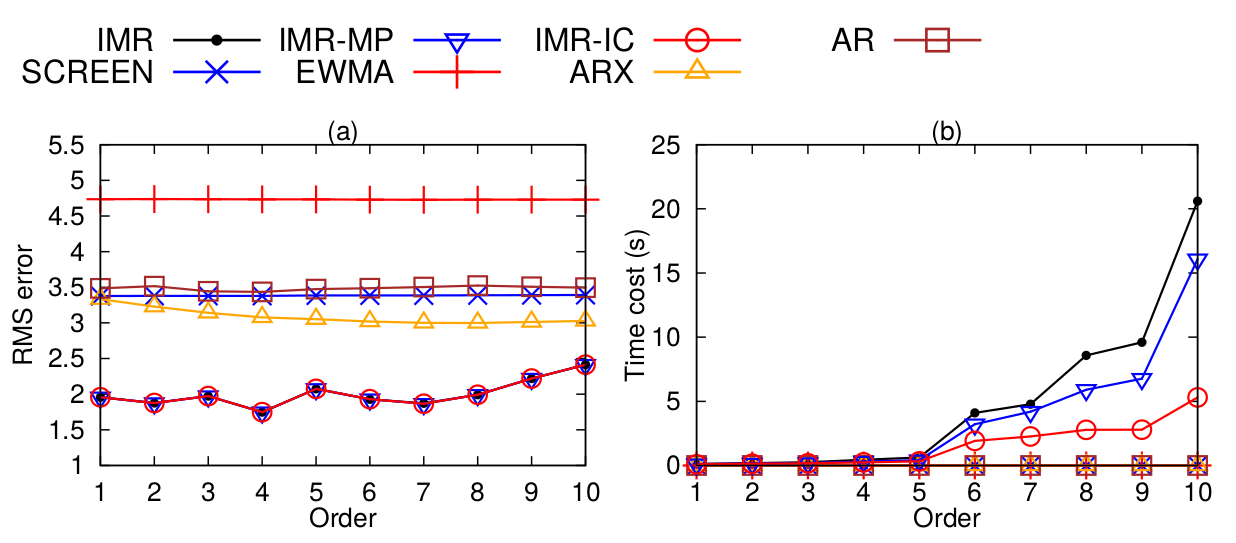
\includegraphics[width=\textwidth]{../plots/varying_order_p.png}
    \caption{Unterschiedliche Ordnung $p$ über GPS-Daten mit $\tau$ = 0.2, Datengröße 750 und Markierungsrate 0.2}%
    \label{varying_order_p}
\end{figure}
\begin{figure}[htbp]
    \centering
    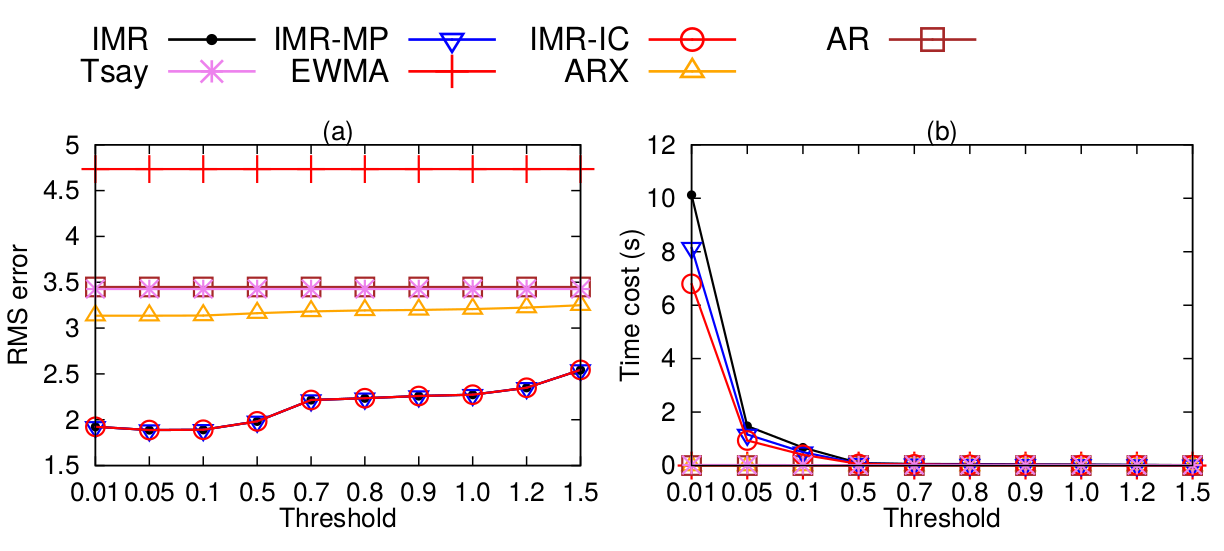
\includegraphics[width=\textwidth]{../plots/varying_threshold.png}
    \caption{Unterschiedliche Schwellenwerte $\tau$ über GPS-Daten mit $p$ = 3, Datengröße 750 und Markierungsrate 0.2}%
    \label{varying_threshold}
\end{figure}
\begin{figure}[htbp]
    \centering
    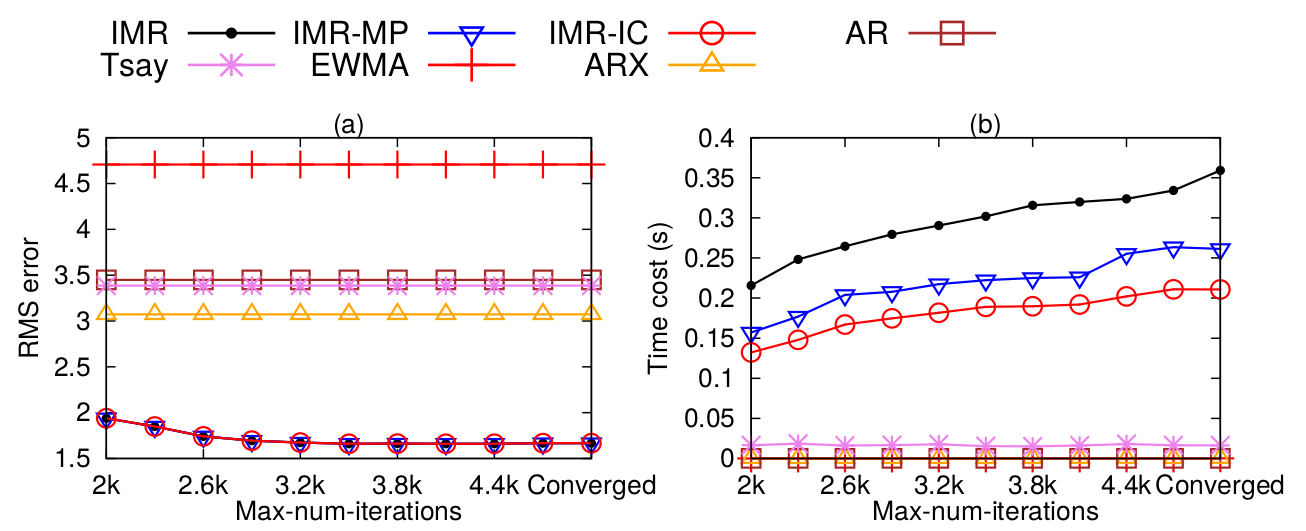
\includegraphics[width=\textwidth]{../plots/varying_maximum_number.png}
    \caption{Unterschiedliche maximale Anzahl von Iterationen über GPS-Daten mit $\tau = 0,2$, $p$ = 3 und Datengröße 750}
    \label{varying_maximum_number}
\end{figure}
\begin{figure}[htbp]
    \centering
    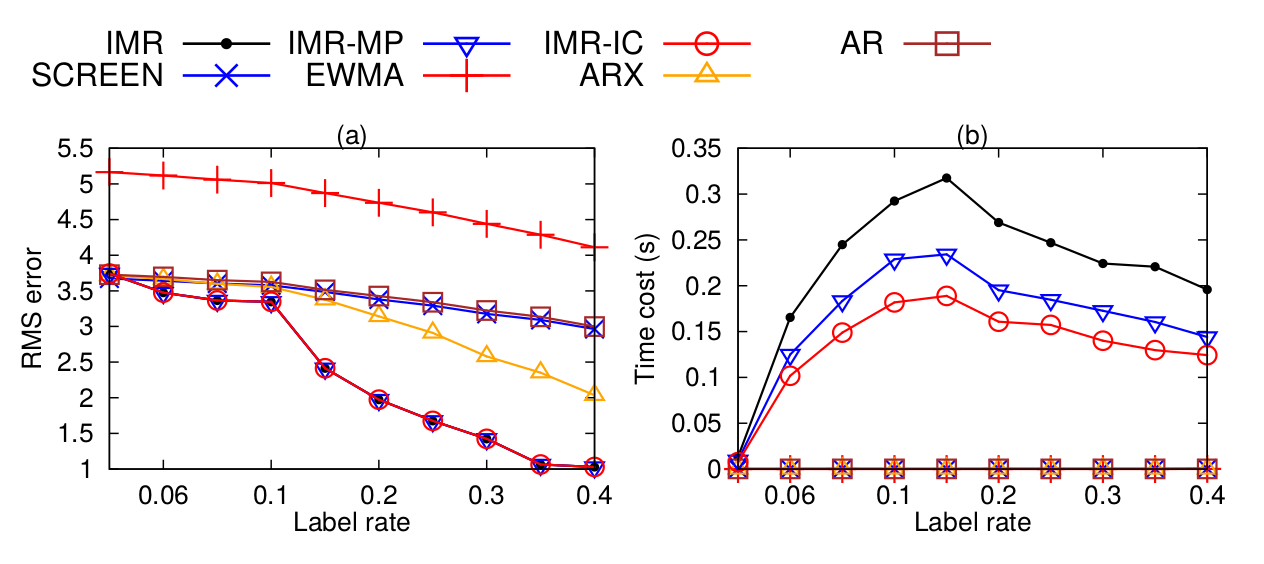
\includegraphics[width=\textwidth]{../plots/varying_labeling_rate.png}
    \caption{Unterschiedliche Markierungsraten über GPS-Daten mit $\tau = 0,2$, $p$ = 3 und Datengröße 750}
    \label{varying_labeling_rate}
\end{figure}

% At the end, there is a final section concluding and summarizing a paper, putting the entire work into perspective and explaining, on a larger level, what the consequence of the models/approaches/methods are and how this answers the research question that has been raised in the introduction.
Erkennung und Bereinigung von Anomalien ist ein sehr schweres Problem. In ein
System können Fehler  aus unterschiedlichen Quellen und zur
unterschiedlichen Zeiten auftreten. Daraufhin wird dieses Problem
eingeschränkt, indem man Zusätzliche Informationen, wie die im Vorfeld richtige
Kennzeichnung der Werte, ausnutzt. 

Bedingungsbasierte Verfahren nutzen keine vollständige temporäre
Eigenschaft der Zeitreihen aus, dennoch wenden das
Minimum-Change-Prinzip an. Im Gegensatz, Modelle, die die Historie der Daten 
nutzen, wie AR oder ARX, implementieren das Minimum-Change-Prinzip nicht.
Darüber hinaus können AR und ARX modifiziert werden um die erkannte Anomalien
zu korrigieren, leider können diese Modelle Daten deutlich ändern. Im Paper
wird IMR vorgestellt, welche beide Ansätze implementiert. Durch die minimale
Änderungen der Daten (nach jede Iteration), ergibt sich eine höhere Genauigkeit
in der Auswertung der Reparation. Danach gehen die Autoren noch eine Stufe weiter und
entwerfen zwei weitere Erweiterungen um die Komplexität von IMR erheblich zu
reduzieren, ohne die Genauigkeit zu beeinträchtigen. Am Ende zeigen die
Experimente, wie die Metaparametern sich zu RMSE und Laufzeit verhalten.
Interessanterweise der Parameter $p$ aus $ARX(p)$ braucht ein niedrigen Wert um
höhe Genauigkeit zu erlangen.

Schlussendlich in diesem Paper wird nur über lineare Modelle gesprochen. Oft
hat man das Problem, dass Datensätze nicht linear abzubilden sind. Ein
interessanter Versuch wäre mit unterschiedliche Modelle IMR zu implementieren.
Als Beispiele könnte man ein Auto-Encoder entwickeln, welcher aus der Daten
eine nicht lineare Rekonstruktion lernt. Dazu könnte man die markierte Daten
benutzen um das Modell online zu trainieren um die Genauigkeit der Reparation
zu erhöhen.


%%%%%%%%%%%%%%%%%%%%%%%%%%%%%%%%%%%%%%
%\bibliographystyle{apa}
\bibliographystyle{ieeetr}
\addcontentsline{toc}{section}{References}% Add to the TOC
%source for the reason we used roulette AND tournament selection
%https://www.hindawi.com/journals/mpe/2016/3672758/
\bibliography{bib}
%\printglossary
\end{document}


